\section{Results}
\labsec{results}

\subsection{Nested Cross-Validation Package}

All the similar published works use a 5-fold cross-validation to 
evaluate their models. However, since there are also some parameters to 
tune, they rely on a (computationally expensive) netsed cross-validation 
in order not to overestimate the predictive power. Since I needed to run 
several different models for each of the 140 genes, each with its own 
parameters, I decided to write an R 
package\sidenote[][-2.3cm]{\url{https://github.com/fmarotta/cvtools}} to 
perform the nested cross-validation with a heuristic algorithm that does 
not try all the possible values for the parameters, but rather, 
independently for each parameter, it starts at one value and explores 
the adjacent ones; then, it moves in the direction where the error 
decreases
(\reffig{cv}).

\begin{marginfigure}[-3.4cm]
  \centering
  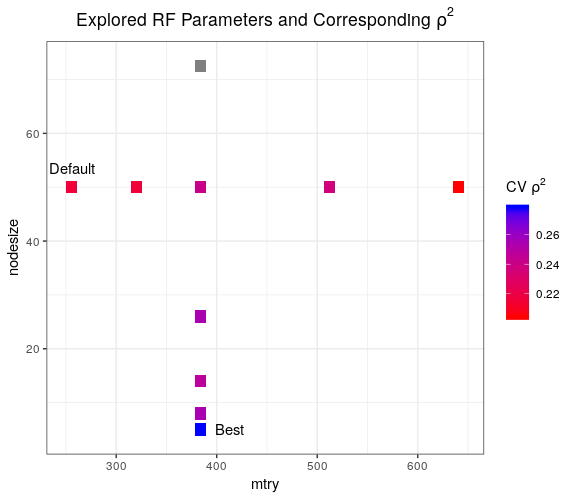
\includegraphics{cv}
  \caption{First, the mtry is tuned while the nodesize is kept fixed; 
the algorithm started at the default value of 256, then it moved up in 
the range as long as the error decreased, and finally it came back to 
explore the values in between. Next, the nodesize was tuned in a similar 
fashion.}
  \labfig{cv}
\end{marginfigure}

This package requires the user to write a function which takes 
predefined arguments and returns a predefined output, but except for 
that, it can be used with any regression model. I evaluated the 
performances of ridge, BART, random forest, and PCR. 
\sidecite[-12.9cm]{James2013a,Hastie2009}

\subsection{Model Performance}

The measure of performance is not the MSE nor the $R^2$, but rather the 
square of the correlation between true and predicted expression 
($\rho^2$); indeed, we do not want to penalise errors on single 
individuals, but we are interested in the general trend of expression. I 
decided to compare my results with those of TIGAR, \cite{Nagpal2019} 
which is currently most recent paper on this topic.

\begin{table}[b]
  \caption{Mean $\rho^2$ across 141 genes. The t-test was always 
performed with respect to TIGAR.}
  \labtab{comp}
  \begin{tabular}{lcc}
  \textbf{Model} & \textbf{Mean} \boldmath$\rho^2$ & \textbf{t-test pval} \\
  \midrule
  TIGAR & 0.067 & NA\\
  Ridge & 0.076 & 0.025\\
  BART & 0.074 & 0.121\\
  Ranger & 0.069 & 0.398\\
  PCR & 0.064 & 0.737\\
  \end{tabular}
\end{table}

Even if it captures only the linear relationships, ridge gave the best 
predictive performance (\reffig{rho2distr}), probably because in this 
context where $p >> n$, it is a good compromise between bias, variance 
and overfitting. According to a t-test, the $\rho^2$ achieved by ridge 
with the TBA values are even higher than those obtained by TIGAR 
(\reftab{comp}).

\begin{marginfigure}[-2cm]
  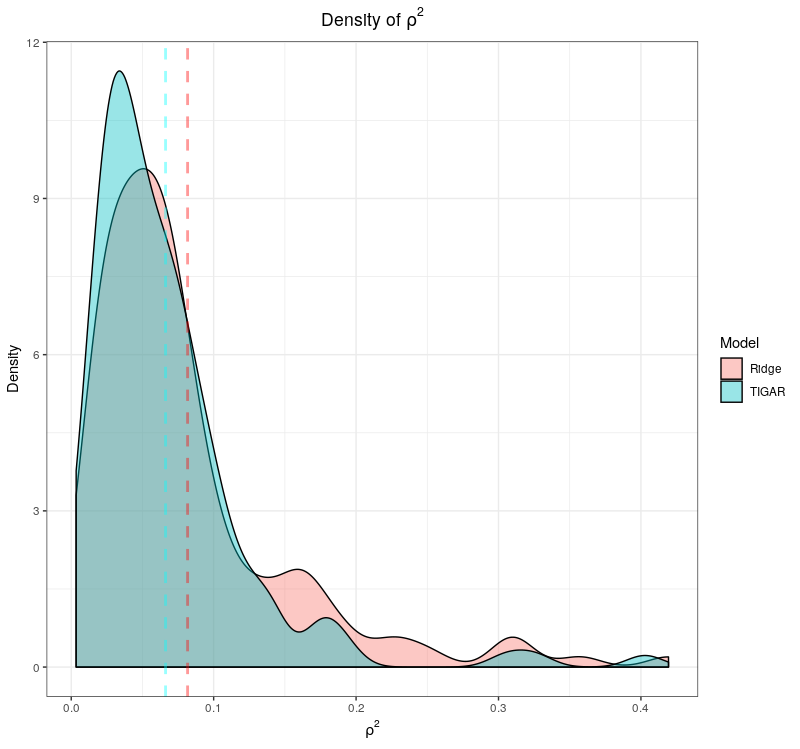
\includegraphics{rho2distr}
  \caption{Density plot of the $\rho^2$ achieved by T-REx (Ridge) and 
TIGAR. The dotted lines denotes the means of the 
distributions.}
  \labfig{rho2distr}
\end{marginfigure}

The performance of BART was not so different, despite the method being 
completely different. However, an important advantage of BART with 
respect to ridge is its ability to provide importance measures, allowing 
us to find which transcription factors are important for each gene. 
Additionally, BART captures the interactions between transcription 
factors.

The other methods, random forest and principal component regression, 
were much less powerful.

\subsection{Considering the Expression of the Transcription Factor}

As high as its affinity for the DNA may be, if the transcription factor 
is present only in tiny amounts it will not bind many regulatory 
regions. For this reason, we tried to enhance our predictors with 
information from the expression of the transcription factors.

\marginnote{%
The Hill equation models the rate of expression of a gene:
\begin{equation*}
  \theta = w \frac{L^n}{K^n + L^n} \approx w \left(\frac{L}{K}\right)^n.
\end{equation*}
Here, $L$ is the amount of transcription factor, $K$ is the dissociation 
constant (the inverse of the affinity), and $w$ is a constant. It is 
reasonable to suppose that if many transcription factors regulate a 
gene, the rate will be given by the following product, where we denoted 
$A = 1 / K$:
\begin{equation*}
  \theta = w_1 \left( L_1 A_1 \right)^{n_1} \cdots w_p \left( L_p A_p \right)^{n_p}.
\end{equation*}
Now, if we compute the log of the rate, we get a linear combination 
which in principle is a deterministic function, but in practice we can 
use this linear combination as the right-hand side of a model formula 
and let ridge estimate the coefficients:
\begin{align*}
  Y \sim \beta_0 &+ \beta_1 \left(\log L_1 + \log A_1\right) \\
                 &+ \cdots \\
                 &+ \beta_p \left(\log L_p + \log A_p\right).
\end{align*}
}

In the dataset, we have expression values for some 40.000 genes; of 
these, about 800 are transcriptional factors. In practice we removed 
those rows from the dataset, and summed the TBA and the expression of 
corresponding transcription factors. The new predictors gave a 
considerable improvement in the performance, and, perhaps surprsingly, 
ridge outclassed BART. In the adjacent margin note I describe the 
working hypothesis more in detail.

\begin{table}[H]
  \begin{tabular}{lr}
  \textbf{Model} & \textbf{Mean} \boldmath$\rho^2$ \\
  \midrule
  Ridge & 0.393\\
  BART & 0.268\\
  \end{tabular}
\end{table}

